\chapter{Theory}\label{theory_part}
This chapter covers the various techniques used in image processing, explained in theory but not in practice. Later, in chapter \ref{implementation}, we will return to the Magic Canvas program and explain how those theories were applied and implemented.

\section{A general framework for image processing}
During this third semester project, image processing has been used to achieve the goals of the project.
Image processing is an umbrella term that covers a set of tools used to process images and/or video. \citep{ip_book} writes that image processing comes from the general field of signal processing, and that it covers ways to segment objects of interest in a digital image. This is achieved by using multiple steps. It should be noted that the order of the steps sometimes change and there might be more focus on some steps than others, depending on the specific goal. (see figure \ref{fig:ip_framework}) it shows a general framework that can be used as a good starting point \citep{ip_book}.

\begin{figure}[htbp]
\centering
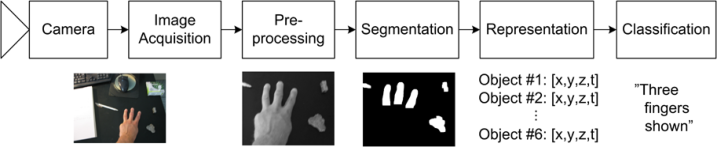
\includegraphics[width=1.00\textwidth]{Pictures/Theory/imageProcessing_steps.png}
\caption{Image Processing framework, from \citep{ip_book}.}
\label{fig:ip_framework}
\end{figure}

\textbf{Image Acquisition}
Before anything can be processed, data needs to be captured, typically using a camera. This step is all about the setup, as well as the environment, setting, lighting and so on.

\textbf{Pre-processing}
Here the initial arrangement is completed, e.g. converting the image from color to grayscale.

\textbf{Segmentation}
To be able to work with a specific object, it needs to be separated from the rest of the picture. This is done using segmentation to remove noise and background elements, so that only the object of interest is seen. Thresholding is often applied to make the object stand out, i.e. make the object appear white and the background black.

\textbf{Representation}
The object needs to be represented in an intuitive manner.

\textbf{Classification}
For the system to actually know if an object is a hand or not, it has to do some features extraction and classifications to compare the data to some predefined database. This can be done with template matching and BLOB classification.

%% Maybe a little too blabla and too long sentences - Gustav %%
%% I moved a paragraph to the begining of the section and changed some things. But I'm still not sure if the above part is useful, as we will be describing everything again... - Marta %%

The combination of these different techniques makes it possible to get a functional program, but before using them, it is necessary to know how they work. The following sections will explain the different techniques in theory, starting with a basic information about digital image acquisition.

\section{Image acquisition}

An image captured through a camera is the result of reflected light being detected on a camera sensor, (see figure \ref{fig:light_cam}). This process is know as \textit{image acquisition}. In this section the basics of image acquisition using a digital camera will be explained. Though it is necessary to have a basic understanding of the physics behind light to get through this process.

\begin{figure}[htbp] 
\centering 
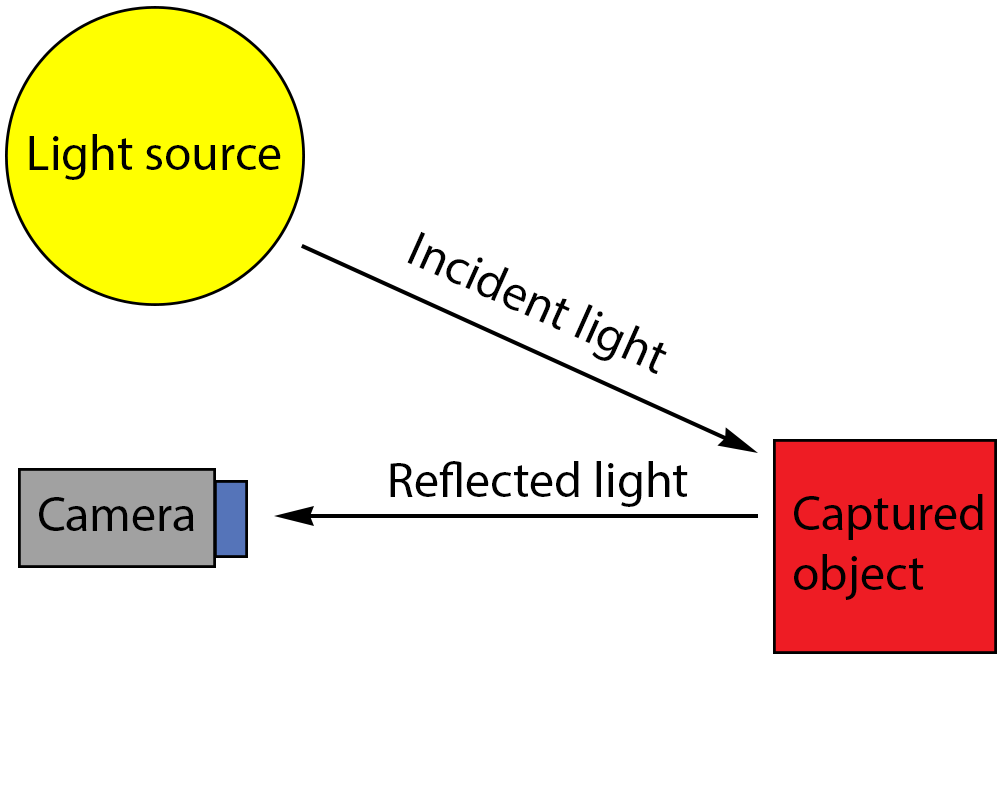
\includegraphics[width=0.5\textwidth]{Pictures/Theory/light_from_sun.png} 
\caption{Light as captured by a camera} 
\label{fig:light_cam} 
\end{figure}

Light is a form of electromagnetic radiation that can be viewed as both waves and particles. This duality is however not something that will be covered within this section, as the wave model is sufficient to build the foundation of the understanding we need. A light wave is a small packet of energy travelling through space. These energy packets are known as photons and they can be described by three properties:

\begin{itemize}
\item \textbf{Wavelenght} - Measured in meters from wave top to wave top and denoted as $\lambda$.
\item \textbf{Frequency} - Measured in oscillations per second, Hz, denoted $f$.
\item \textbf{Energy} - Measured in electronvolts, eV, denoted $E$.
\end{itemize}

To derive the wavelength or the frequency, formula \ref{eq:wavelenght} is applied:
\begin{align}
\centering 
\lambda = \frac{C}{f}
\label{eq:wavelenght} 
\end{align}
where {$C$} is the speed of light.

The wavelength of the photon determines what color will be perceived. As the speed of light is constant, changing the frequency will alter the wavelength. When photons impact objects, the material provokes a refraction that changes the frequency of the wavelength and therefore, a color can be perceived. The visible spectrum of light is only a fraction of the full spectrum of electromagnetic radiation, (see figure \ref{fig:em_rad}). Light interacts additively, with a mix of equal parts of each wavelength resulting in white light. The light from the sun can be broken down into its component wavelengths by refracting the light in a prism. This yields the full spectrum of visible light, as seen in a rainbow.

\begin{figure}[htbp] 
\centering 
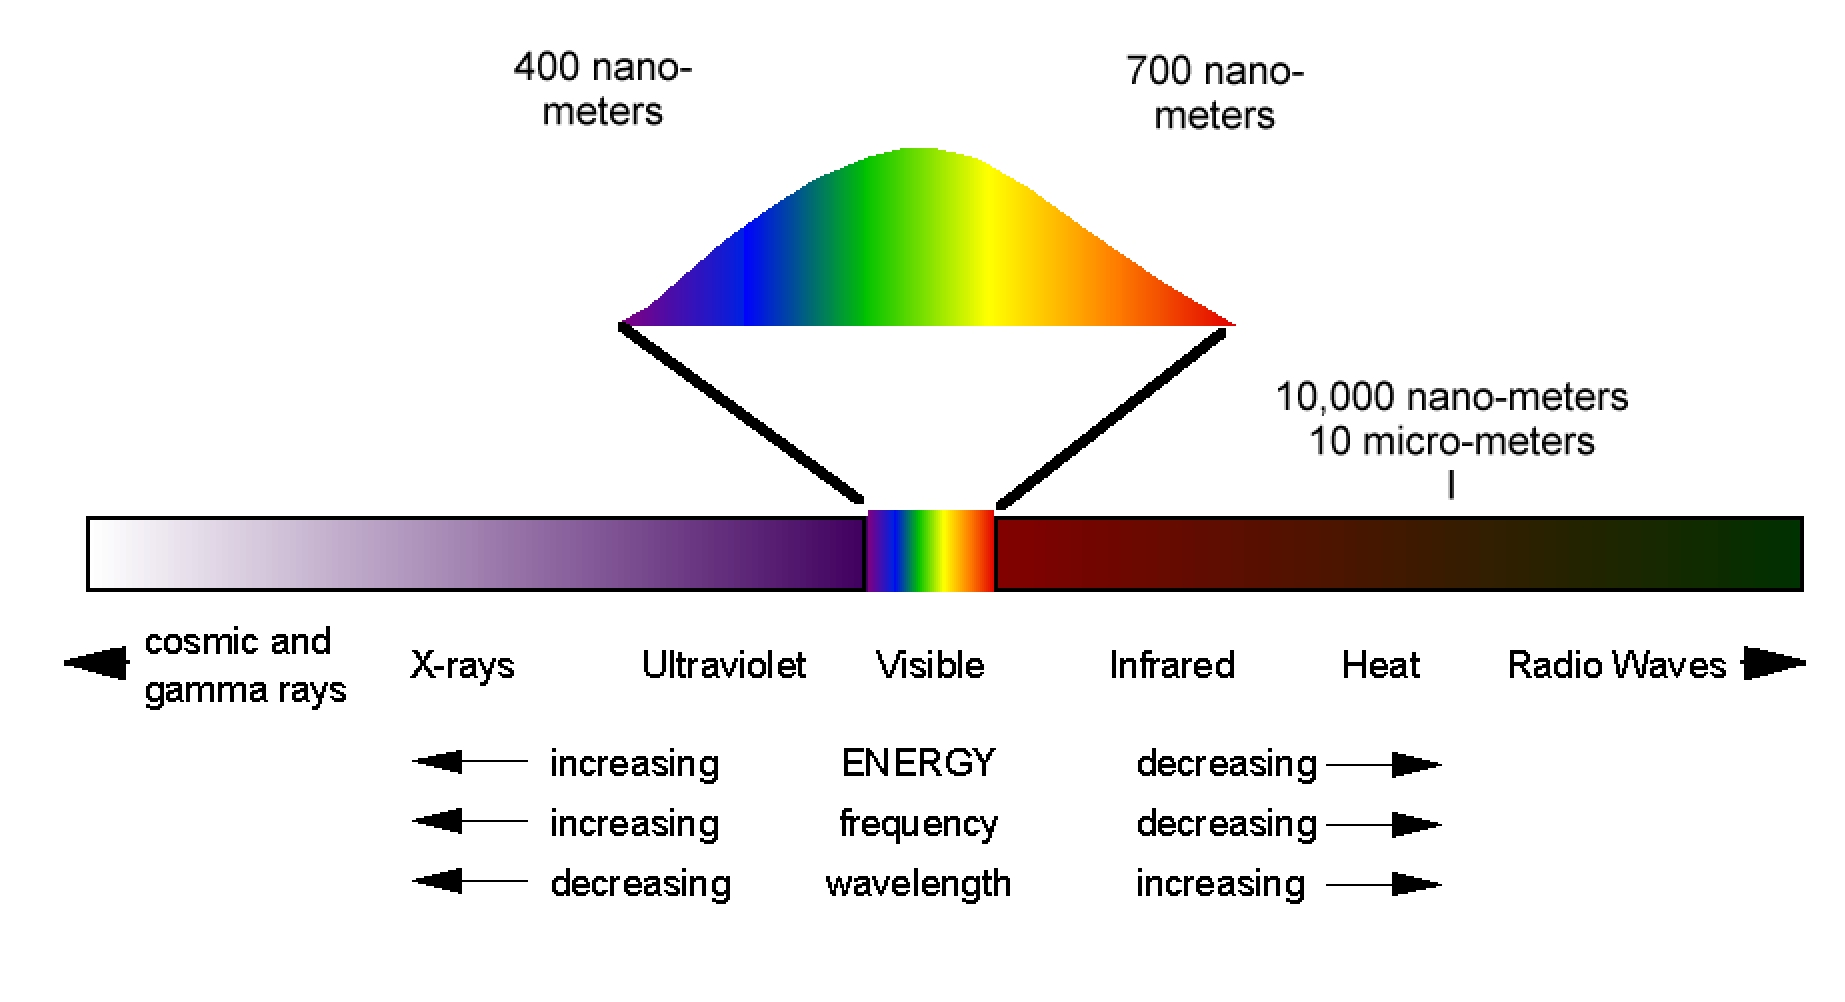
\includegraphics[width=1\textwidth]{Pictures/Theory/em_rad.png} 
\caption{Figure illustrating the full spectrum of electromagnetic radiation.} 
\label{fig:em_rad} 
\end{figure}

\subsection{Digital image acquisition}
When capturing an image using a digital camera, light passes through a lens onto the sensor. This acts in much the same way as the human eye. In place of photoreceptors sensitive to specific wavelengths, a camera sensor has a physical matrix of pixel sensors (one for each pixel in the output image). A camera that can capture color images has three types of sensors in each pixel\citep{ip_book}.

\section{Digital images}
One does perhaps not realize the technical aspects happening when capturing an image with a camera. In fact, several different computations are happening simultaneously. To be able to get some useful information from images and use it for further purposes, such as altering the image in an image editing program, it is necessary to have some fundamental knowledge about how images work on a computer. (see figure \ref{fig:ip_ColoredToGrayscaleToBinary}) it shows what this chapter is all about: working with color, grayscale, and binary images, as well as the different attributes of each type.

\begin{figure}[htbp]
\centering
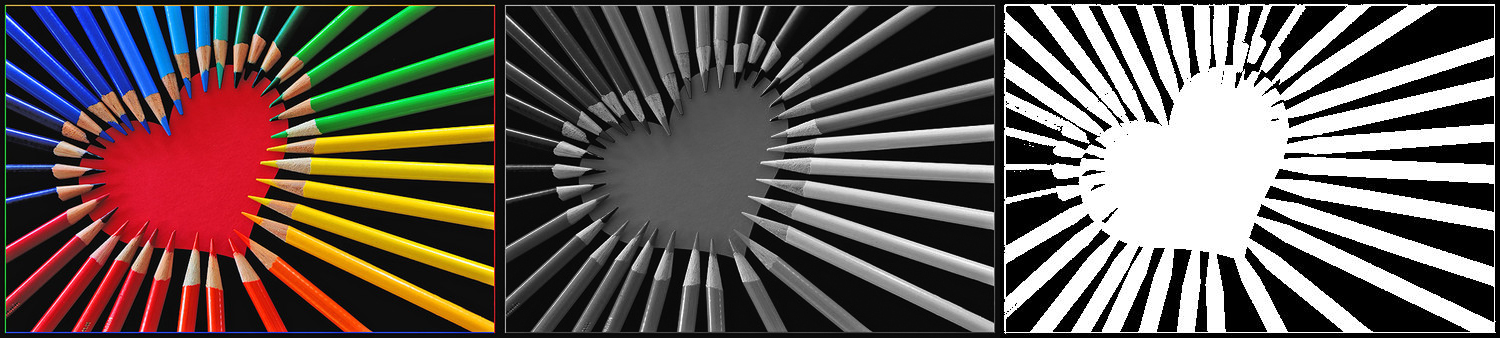
\includegraphics[width=1.00\textwidth]{Pictures/Theory/ColoredToGrayscaleToBinary.jpg}
\caption{Image illustrating a conversion from a color image to grayscale and finally binary. Inspired by \citep{colorPencils}.}
\label{fig:ip_ColoredToGrayscaleToBinary}
\end{figure}

\subsection{Pixels}
When a digital camera takes a picture, it uses an image sensor consisting of an array of interconnected cells. All cells hold a filter and a sensor. As light hits the cells, the energy is converted into a digital number via an analog-to-digital converter (ADC). This value is denoted a \textit{pixel} and describes how bright a specific part of the image is \citep{ip_book}.

\subsection{Bits and bytes}
The way computers store data is using bits and bytes. One bit can be thought of as a switch that can be turned on or off. However, instead of on/off buttons, a computer uses digits in form of 0's and 1's. A byte consist of 8 bits and is a row of eight "switches" capable of holding the values 0 and 1. This provides one byte with the ability to store 256 different values, since $2^{8}$ is equal to 256. 

%Figure \ref{fig:bits} displays the concept behind bits and bytes. To give an example of how a byte could be used, this \href{http://www.asciitable.com/}{ASCII table} shows that the letter 'K' has the number 107. To write 'K' in binary, the byte has to equal to 107 using all 8 bits. It would be written in binary form like this: 0110100.

%The reason is that (0*128)+(1*64)+(1*32)+(0*16)+(1*8)+(0*4)+(1*2)+(1*1)=107

%\begin{figure}[htbp]
%\centering
%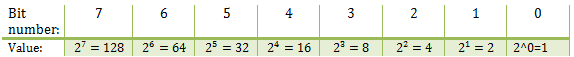
\includegraphics[width=1.0\textwidth]{Pictures/Theory/BitAndByte}
%\caption{When reading bits, you start from right and go left. Each value is in the power of two.}
%\label{fig:bits}
%\end{figure}

\subsection{8-bit images and grayscale images}
In an 8-bit image, the 8-bit prefix describes the \textit{bit depth} of the image. The bit depth tells us about the amount of information that can be stored in a single pixel.

%The hue defines how pure and vivid a color is \citep{visual_story}. 

An image with a single channel of information for each pixel in the X and Y axis is typically a grayscale image. The information stored in each pixel is the gray-level value of the particular pixel \citep{ip_book}. Considering an 8-bit image, each pixel can hold 256 different levels of gray. In the case of a zero-based computer system, this equates to a pixel holding a value between 0-255 (see figure \ref{fig:ip_grayscale}). While 8-bit images are widely-used as a format for images, it is also possible to create images capable of holding more than 256 gray-level values for each individual pixel.

\begin{figure}[htbp]
\centering
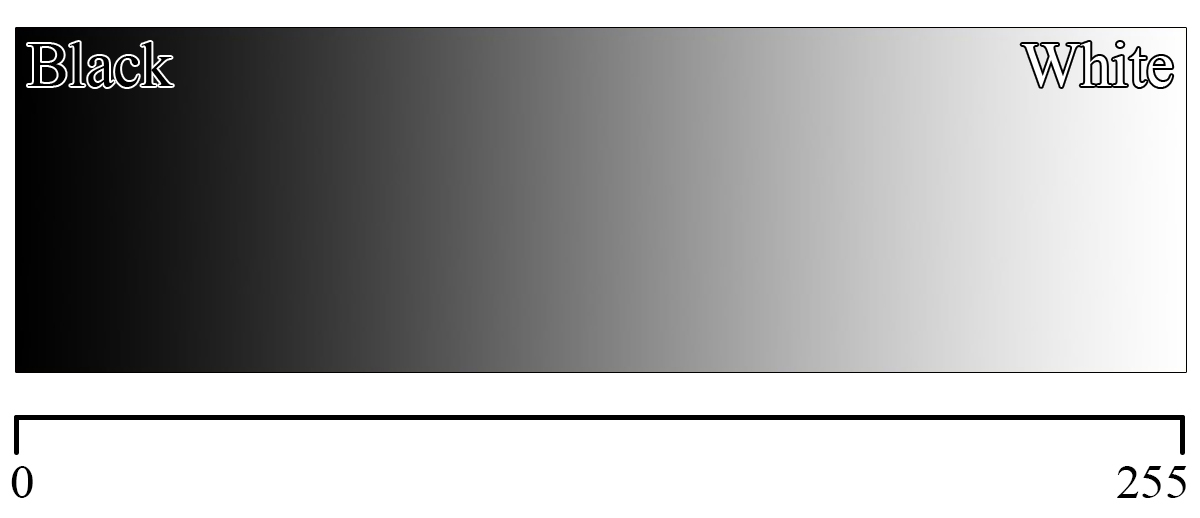
\includegraphics[width=0.7\textwidth]{Pictures/Theory/Grayscale.jpg}
\caption{Image illustrating the 256 different gray-level values of an 8 bit picture.}
\label{fig:ip_grayscale}
\end{figure}
 
\subsection{Indexing an image}
When working with images on a computer and performing image processing, one often has to look at the individual pixels within an image.

Working with pixels in an image is similar to working with a coordinate system. The image is indexed from the top-left corner. Both X- and Y-axes are indexed beginning with (0,0). Going to the right the X value increases, going down the Y value increases. A single pixel can be described as a coordinate, e.g. (see figure \ref{fig:ip_IndexingAPicture}) the pixel (1191,665) is the bottom-most corner to the right.

\begin{figure}[htbp]
\centering
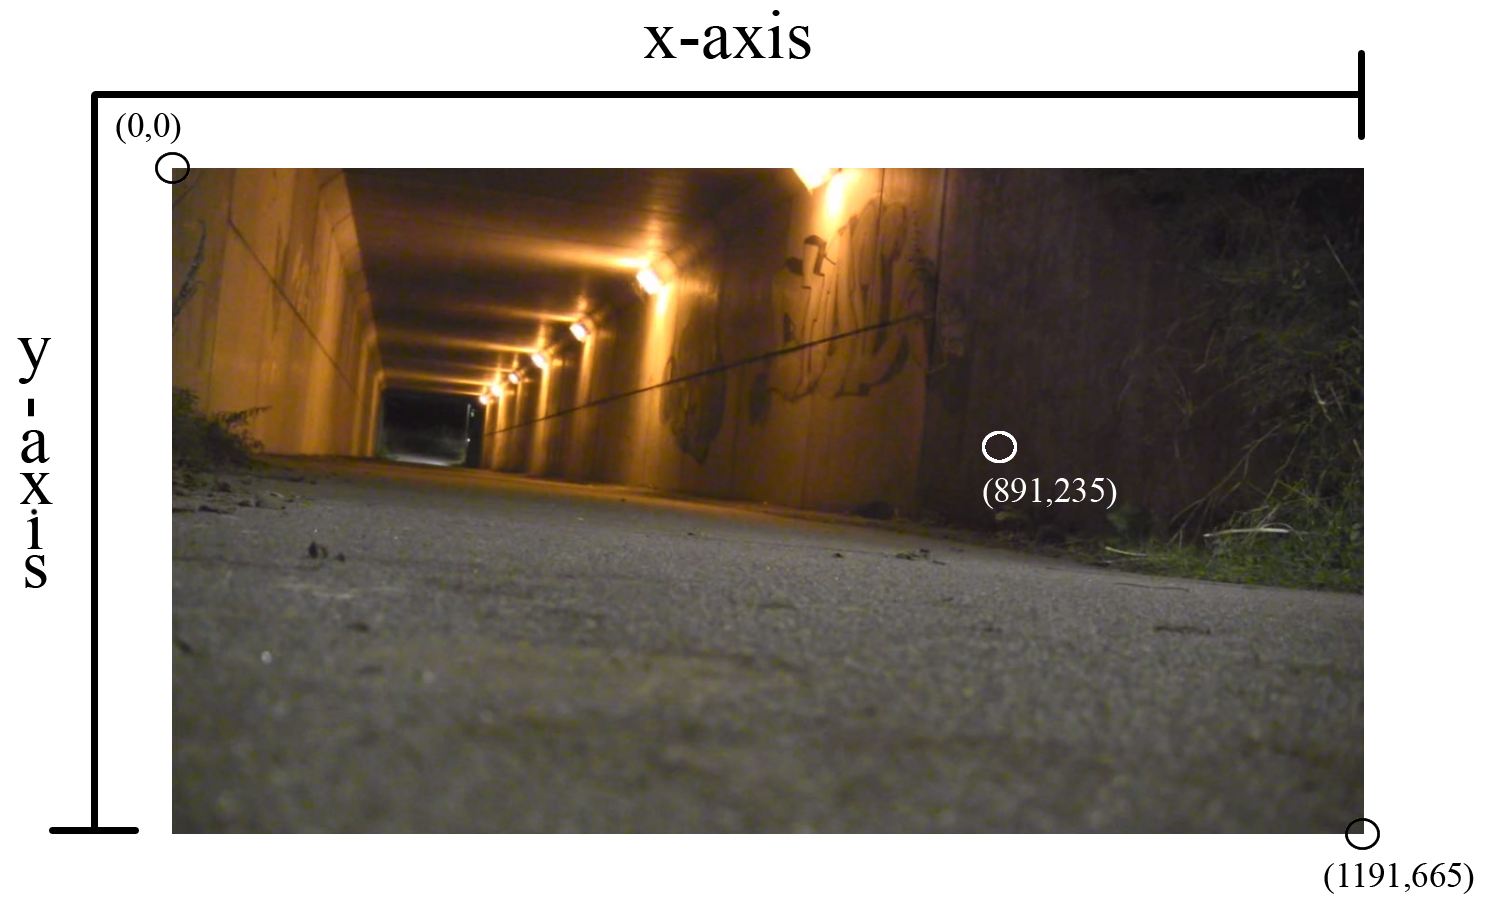
\includegraphics[width=1.00\textwidth]{Pictures/Theory/IndexingAPicture}
\caption{The pixel values are stored in a coordinate system. Note that the Y-axis is reversed.}
\label{fig:ip_IndexingAPicture}
\end{figure}

\subsection{Working with color images}
Now that a basic knowledge regarding images has been established, the next step into using images in calculations is to understand the basics of a color image.

There are several formats for handling color images. In this report we will only describe RGB (red-green-blue). The main difference when talking about color and grayscale images, is that color images have three channels, compared to the single channel in grayscale images. Each of the three channels holds the value of a specific color for each pixel in red, green and blue, which are the primary colors our eyes are sensitive to. In addition, equal amounts of red, green and blue will produce a gradient of grey. A pixel with each color channels holding a value of 255 produces a white pixel, and a pixel with the color channel values of 0 will produce a black pixel. This  is explained by the additive mixing of colors in RGB images \citep{ip_book}. % To exclude a specific color in a mathematical operation, such as red, it is necessary to use thresholding to segment the pixels depending on values of the red channel (this will be described in \ref{sec:Thresholding}). The outcome in that case would be a picture with a limited/controlled amount of red.

\subsection{Binary images}
In a binary image a pixel is either white or black (true or false). Binary pictures are less resource-demanding when performing mathematical operations as each pixel can take only one of two values.

\section{Segmentation}
Segmenting an image or video is the process of extracting the information you are interested in. Segmentation often consists of different sub operations, all with the same goal of getting the information you want from the input image \citep{ip_book}. Before segmentation is applied, an image undergoes preprocessing. This might be converting from a color image to a grayscale image to ease the computations required. (see figure \ref{fig:ip_ColoredToGrayscaleToBinary}) It serves as an illustration of preprocessing and segmentation. First the image is converted to a grayscale image, this step is part of the preprocessing. Then the image is thresholded, which yields a binary image with only the pens and the heart. 

Two possible problems can arise while segmenting an image. If the segmentation algorithms are too strict, and do not include enough in their extraction, the object meant to be extracted might not be complete. Therefore it might not be recognized correctly. This case is called \textit{under-segmentation} \citep{ip_book}.

In the opposite case, the algorithm is too sloppily designed. The result is that too much of the input image is included in the segmentation. The final segmented image might contain too much noise or objects might be connected, even though they were separate entities. This is called \textit{over-segmentation} \citep{ip_book}.

\section{Histograms}
A commonly-used tool when working with digital images is the histogram. Essentially a histogram provides data distribution, which is an easy way to get an overview of the frequency of events. An image histogram is a graphical representation of how many times a specific pixel value appears. This can be used to show whether an image is too dark or too bright, as well as how good the contrast is \citep{ip_book}. (see figure \ref{fig:SimpleThreshold}) It shows a histogram with pixel values from 0-255. The more often a specific pixel value is present on the image, the taller the bin representing what the particular pixel value will be.

\begin{figure}[htbp] \centering
\begin{minipage}[b]{0.45\textwidth} \centering
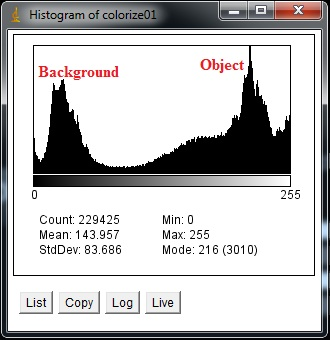
\includegraphics[width=1.00\textwidth]{Pictures/Theory/SimpleThresholdPicture} % Venstre billede
\end{minipage} \hfill
\begin{minipage}[b]{0.45\textwidth} \centering
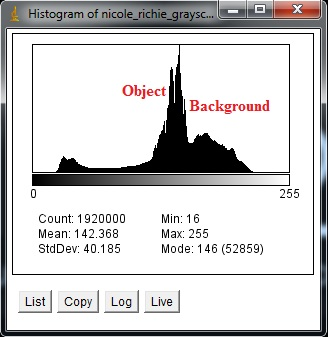
\includegraphics[width=1.00\textwidth]{Pictures/Theory/ComplicatedThresholdPicture} % Højre billede
\end{minipage} \\ % Captions og labels
%\end{figure}
\begin{minipage}[t]{0.45\textwidth}
\caption{Ideal histogram with two "mountains".} % Venstre caption og label
\label{fig:SimpleThreshold}
\end{minipage} \hfill
\begin{minipage}[t]{0.45\textwidth}
\caption{Problematic histogram.} % Højre caption og label
\label{fig:ComplicatedThreshold}
\end{minipage}
\end{figure}

Histograms can also be used to describe the contrast in an image. The contrast is a measure of the difference of intensity levels between the dark and light areas on the picture \citep{histogram}. This means that a histogram with a broader distribution of values will represent an image with good contrast. On the other hand, if the histogram is very narrow, the contrast in the image is smaller, and it will appear more flat and dull (see figure \ref{fig:histogram_contrast}).

\begin{figure}[htbp]
\centering
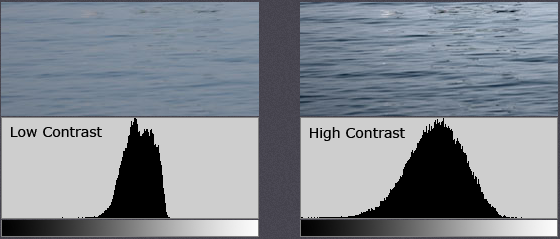
\includegraphics[width=0.80\textwidth]{Pictures/Theory/hisogram_contrast.png}
\caption{Histograms can be used to describe the contrast in an image. Picture from \citep{histogram}.}
\label{fig:histogram_contrast}
\end{figure}

\section{Thresholding}\label{sec:Thresholding}
Thresholding is one of the most fundamental operations when working with images. It is performed to convert an image to a binary image. This is useful in programs where you need to find silhouettes, such as tracking a person, where smaller details are not important.

To determine which pixels should be completely black and which should be completely white, a \textit{threshold value} is required. Using a metaphor, the threshold value can be compared to a gatekeeper that lets everyone who is 18 years old or older inside the club, but denies access to people who are 17 or younger. Using this analogy, pixels that are "old" (bright) enough are let in, while "younger" pixels (dark) are denied. The value used to classify which persons (pixels) can pass and which have to stay out, have to be decided by the gatekeeper (or the programmer, in this case).

In practice this means that pixels with values greater than a threshold is set to true (or white), which typically is 255 when talking in bytes. On the other hand, if a pixel is less than the threshold value, it is set to false (black) or 0. The formula for calculating a threshold is shown in equation \ref{threshold}.
\begin{equation}
  \begin{aligned}
  	\text{if } f(x,y)\leq T \quad \text{then } g(x,y)&= 0 \\
  	\text{if } f(x,y)>T \quad \text{then } g(x,y)&= 255
	\label{threshold}  
  \end{aligned} 
\end{equation}
Where $T$ is the threshold value, $f(x,y)$ is the input pixel and $g(x,y)$ is the output pixel. 

When setting the threshold value it is important to consider what you want as the output. The effect of thresholding will differ from image to image, depending on the contrast between the object and the background. If the background and the object have a high contrast or are very different in color, it will be easy to distinguish them and choose an effective threshold value. However, if the object and background are very similar, it will be hard to choose a value to separate them properly. At that point it will be necessary to choose between losing information associated to the object of interest, or to gather some background noise to preserve it.

Figures \ref{fig:SimpleThreshold} and \ref{fig:ComplicatedThreshold} show the threshold value used on the images \ref{fig:SimpleThresholdAfter} and \ref{fig:ComplicatedThresholdAfter}. Looking to the histograms, it is easy to tell that the leftmost is more ideal to threshold because the object and background are very different. That is shown graphically with two "mountains" in the histogram (see figure \ref{fig:SimpleThreshold}), also called a \textbf{bi-modal histogram} \citep{ip_book}. The effect of a good threshold value can be seen on picture \ref{fig:SimpleThresholdAfter}, where the output gives a clear outline of the silhouette of the woman. On the other hand, the histogram to the right does not have two clear mountains, but a big one and two smaller. This means that the color values are distributed more equally and therefore, it will be hard to define a good threshold value. The result in this case is a poor silhouette of the woman (see figure \ref{fig:ComplicatedThresholdAfter}), due to the fact that the background and the object are too similar.

%Looking at picture \ref{fig:SimpleThresholdAfter} will show that the picture with the leftmost histogram, figure \ref{fig:SimpleThreshold}, gives a clear outline of the silhouette of a woman after the thresholding value is applied. However, looking at figure \ref{fig:ComplicatedThresholdAfter} shows that the picture with the rightmost histogram, figure \ref{fig:ComplicatedThreshold}, produces a poor silhouette of a woman, due to the fact that the background and the object has very similar colors. 

\begin{figure}[htbp] \centering
\begin{minipage}[b]{0.45\textwidth} \centering
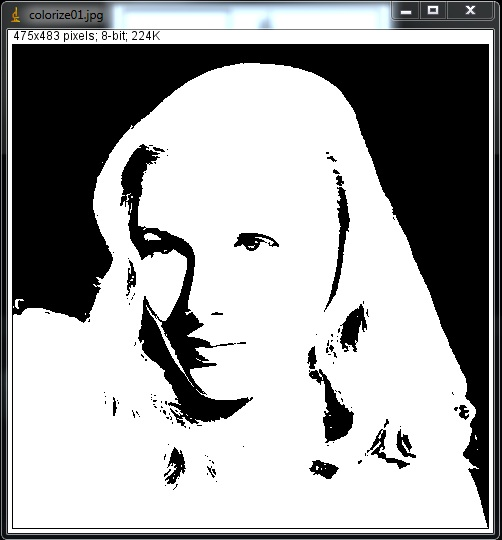
\includegraphics[width=1.00\textwidth]{Pictures/Theory/SimpleThresholdAfter} % Venstre billede
\end{minipage} \hfill
\begin{minipage}[b]{0.45\textwidth} \centering
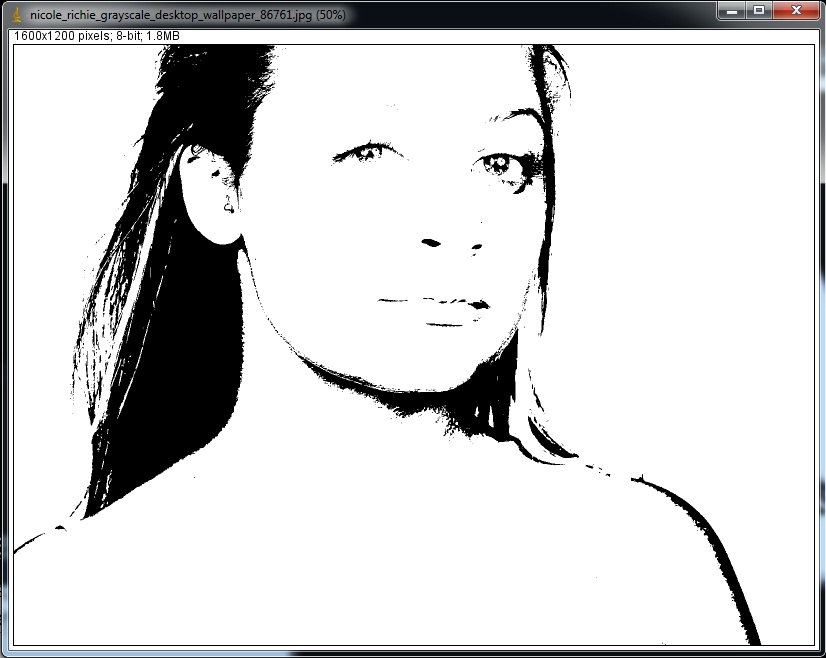
\includegraphics[width=1.00\textwidth]{Pictures/Theory/ComplicatedThresholdAfter} % Højre billede
\end{minipage} \\ % Captions og labels
\begin{minipage}[t]{0.45\textwidth}
\caption{Good silhouette after thresholding.} % Venstre caption og label
\label{fig:SimpleThresholdAfter}
\end{minipage} \hfill
\begin{minipage}[t]{0.45\textwidth}
\caption{Poor silhouette after thresholding.} % Højre caption og label
\label{fig:ComplicatedThresholdAfter}
\end{minipage}
\end{figure}

\section{Morphology}
Morphology is a collection of operations used to analyze and process structures. Although these techniques are commonly used on binary images, it is possible to apply them to grayscale images as well. Morphology on binary images can be used to remove noise produced by thresholding an image, as well as defining the contours of the objects in order to achieve a proper BLOB analysis \citep{ip_book}. BLOBs are described in \ref{blob}.

Morphology is a type of neighborhood processing. In neighborhood processing the surrounding pixels of the input pixel contributes to the operation that is performed on the pixel itself. For this purpose a kernel is used, as shown in figure \ref{fig:kernel}. A kernel, also called \textit{structuring element}, is a grid containing numbers, denoted \textit{kernel coefficients}. These coefficients differ depending on the image processing applied.

\begin{figure}[htbp]
\centering
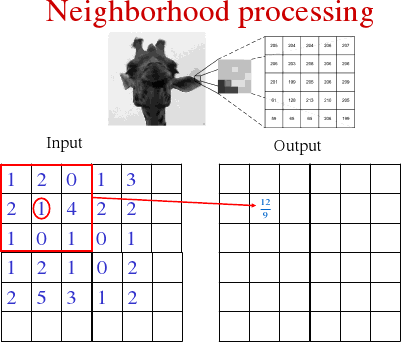
\includegraphics[width=0.7\textwidth]{Pictures/Theory/kernel}
\caption{Neighborhood processing uses a kernel. Image from \citep{ip_book}.}
\label{fig:kernel}
\end{figure}

\subsubsection{Hit and fit}
Whenever one decides to apply a kernel and \textit{hit} or \textit{fit} the pixels, what happens is that the algorithm will compare the values of the pixels on the input image to the kernel. Depending on these values and the image's pixel values, different output occur.

The process of hitting the pixels starts by positioning the kernel on the image, so that it operates on one pixel at a time. If one of the pixels on the input image is a '1' where the kernel is '1' as well, then it is said to hit. This means that the pixel in the center of the kernel will become a '1' (white) in the output. If none of the pixels inside the kernel "hits", then the pixel in the middle of the kernel becomes a '0' (black) in the output.

\begin{figure}[htbp]
\centering
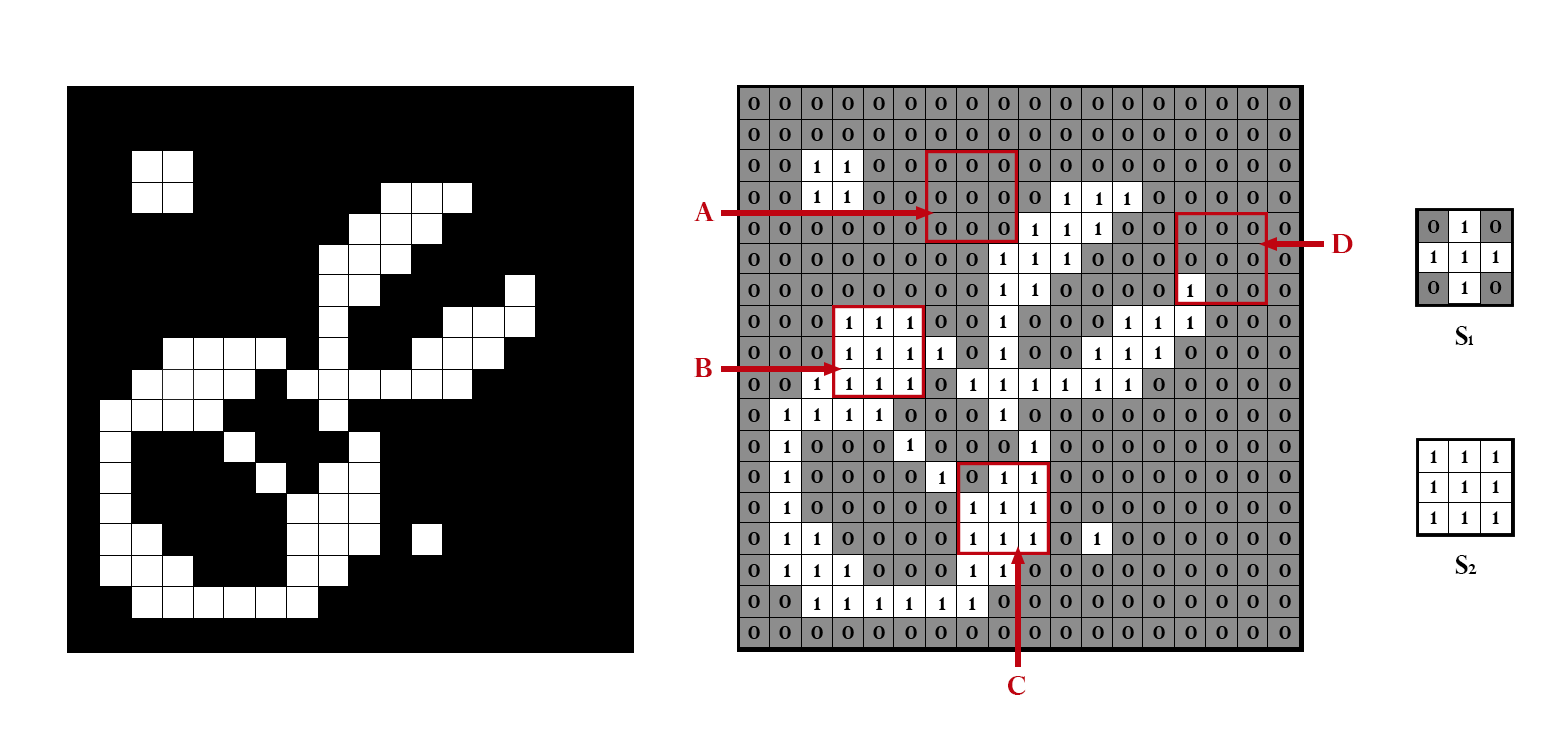
\includegraphics[width=1\textwidth]{Pictures/Theory/FitHitKernels.png}
\caption{Binary image and structuring elements. Inspired by \citep{ip_book}.}
\label{fig:FitHit}
\end{figure}

The opposite operation is fitting the pixels. But in this case, all the values of the pixels on the area of the kernel have to be the same both on the kernel and the input image. If one of the pixels on the input image have a different value to the corresponding 1's of the kernel, the pixel in which the kernel is centred will be a '0' on the output image. On table \ref{tab:HitFitResults} an example image, figure \ref{fig:FitHit}, is being represented with two different types of kernel.
\begin{table}[htbp]
\centering
\begin{tabular}{|c|c|c|c|}
\hline
 \:Position\: &SE &\:\:\:Hit\:\:\: &\:\:\:Fit\:\:\: \\\hline
 \hline
 A &$S_{1}$ &No &No\\\hline
 A &$S_{2}$ &No &No\\\hline
 B &$S_{1}$ &Yes &Yes\\\hline
 B &$S_{2}$ &Yes &Yes\\\hline
 C &$S_{1}$ &Yes &Yes\\\hline
 C &$S_{2}$ &Yes &No\\\hline
 D &$S_{1}$ &No &No\\\hline
 D &$S_{2}$ &No &No\\\hline
\end{tabular}
\caption{Results of hitting and fitting with two different structuring elements. Inspired by \citep{ip_book}.}
\label{tab:HitFitResults}
\end{table}

\subsection{Dilation}
\textit{Dilation} is the process of applying the hit process to an entire image, and it refers to the expansion of an object on an image (see equation \ref{Dilation1} for a mathematical definition). The result of this method implies filling small holes and merging objects. As mentioned before, the final effect on these objects will depend on the kernel, how big it is and which shape it has. This can be seen on figure \ref{fig:Dilation}. 
\begin{equation}
\begin{aligned}
{g(x, y)}={f(x,y)}\oplus{SE}
\label{Dilation1}
	\end{aligned}
\end{equation}
A small kernel applied several times will have the same effect as a big kernel applied once. This can be seen on equation \ref{Dilation2} where dilating twice with the element {$S_{1}$} has the same effect on the object as dilating one time with {$S_{2}$}, even though the only difference between those two kernels is that {$SE_{2}$} has a radius twice times bigger than the radius of {$S_{1}$}.
\begin{equation}
\begin{aligned}
{f(x,y)}\oplus{S_{2}} \approx ({f(x,y)}\oplus{S_{1}})\oplus{S_{1}}
\label{Dilation2}
	\end{aligned}
\end{equation}
%%%%%%%%%%%%%%%%%%%%%%%%% IMAGES WITH DILATIONS %%%%%%%%%%%%%%%%%%%%%%%%%%%%%%%%%%%%
\begin{figure}[htbp]
\centering
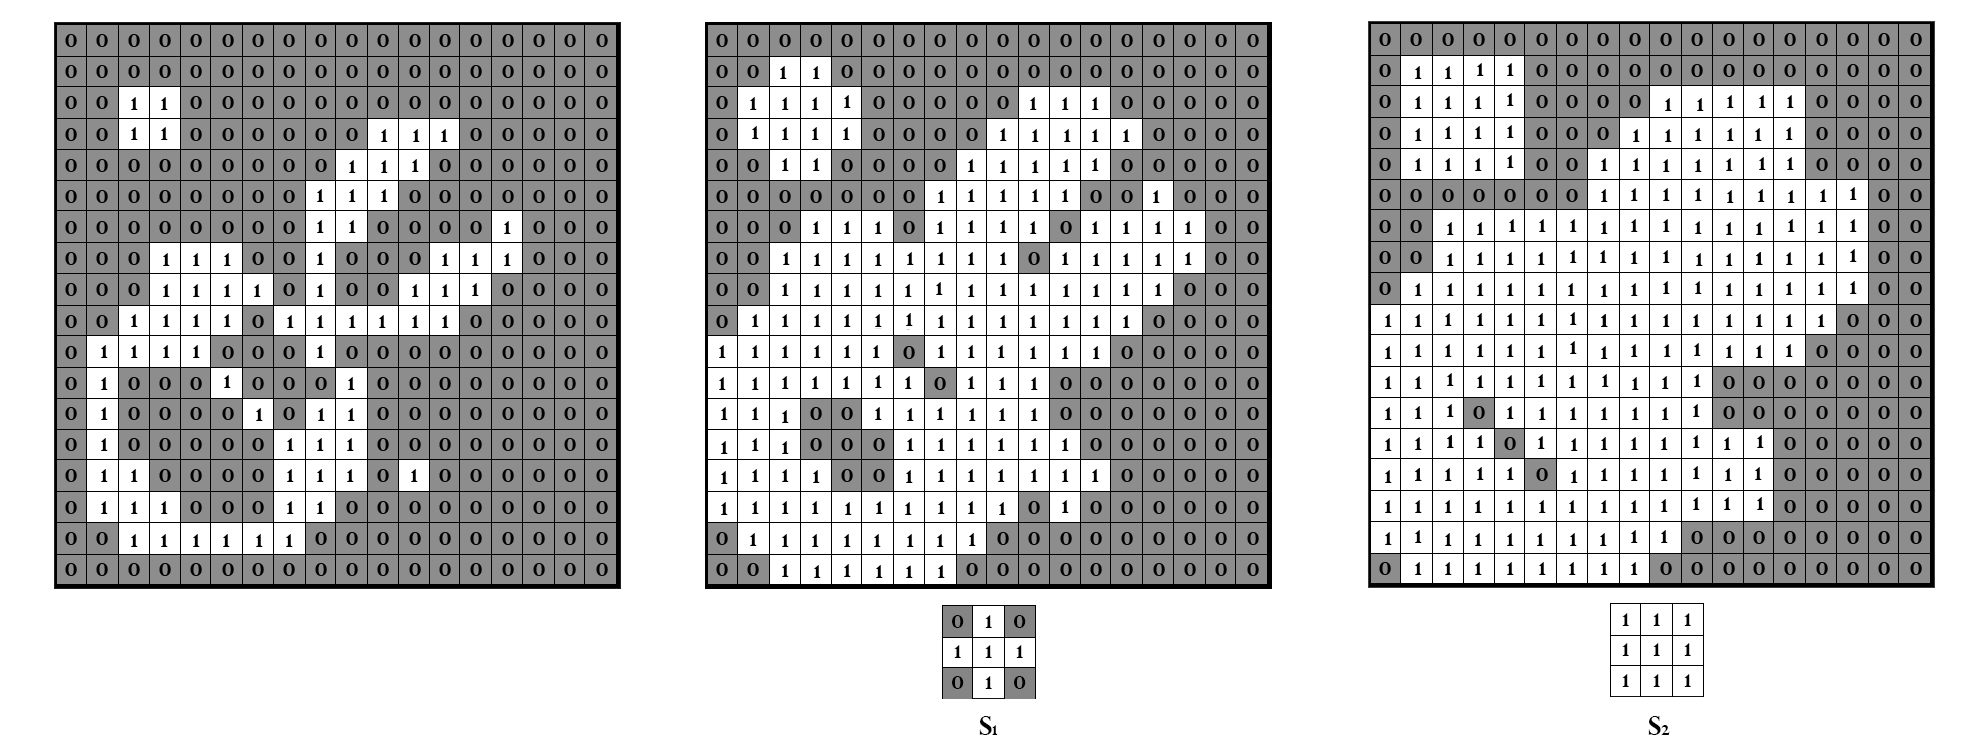
\includegraphics[width=1\textwidth]{Pictures/Theory/Dilation.png}
\caption{Dilation produced by two different kernel. Inspired by \citep{ip_book}.}
\label{fig:Dilation}
\end{figure}

\subsection{Erosion}
\textit{Erosion} is the process of applying fit to an entire image and refers to the reduction of the size of an object in an image (the mathematical definition is provided in equation \ref{Erosion1}). As the fit method is applied, small objects will also disappear and larger objects will be broken down into smaller ones. As it happens with dilation, the effects depend on the size and shape of the kernel.
\begin{equation}
\begin{aligned}
{g(x, y)}={f(x,y)}\ominus{SE}
\label{Erosion1}
	\end{aligned}
\end{equation}

%%%%%%%%%%%%%%%%%%%%%%%%% IMAGES WITH EROSIONS %%%%%%%%%%%%%%%%%%%%%%%%%%%%%%%%%%%%
\begin{figure}[htbp]
\centering
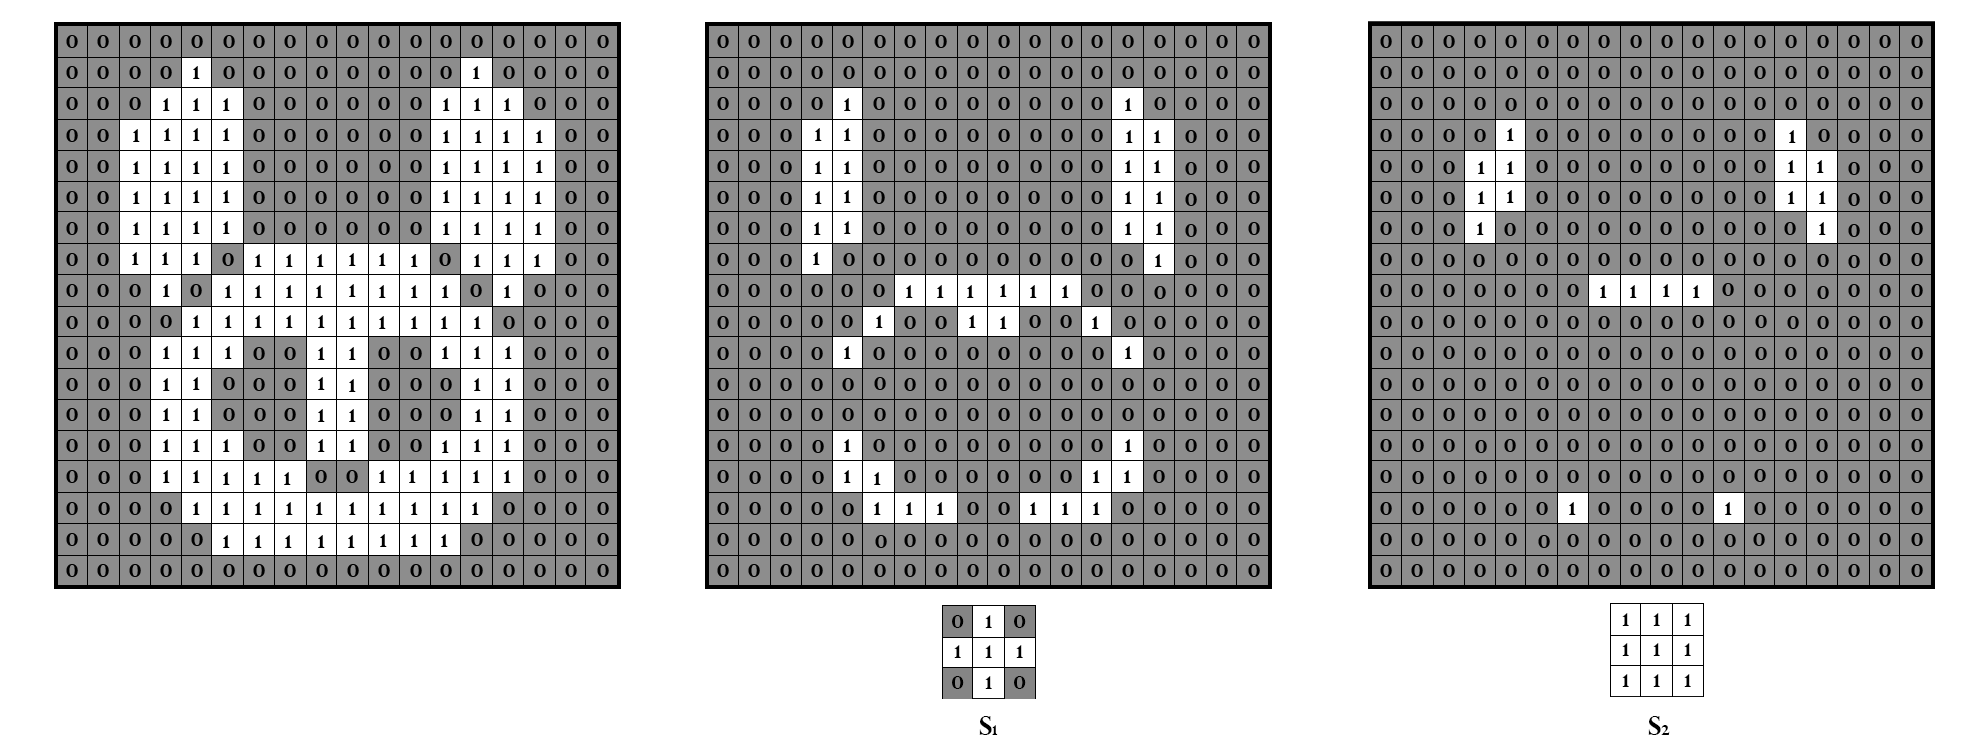
\includegraphics[width=1\textwidth]{Pictures/Theory/Erosion.png}
\caption{Erosion produced by two different kernels. Inspired by \citep{ip_book}.}
\label{fig:Erosion}
\end{figure}

\subsection{Compound operations} \label{compound}
The term \textit{compound operations} refers to the combination of dilating and eroding objects on an image and can therefore imply the \textit{union} or \textit{intersection} of the objects, but also other operations like \textit{closing}, \textit{opening} or doing edge detection, also know as \textit{boundary detection}.
\subsubsection{Opening}
When eroding images to erase noisy objects or split parts, it often occurs that the object of interest has decreased its size. The solution to this problem is to dilate the eroded image. This operation is denoted \textit{opening}, as shown in equation \ref{Opening}.
\begin{equation}
\begin{aligned}
{g(x,y)}={f(x,y)}\circ{SE}=({f(x,y)}\ominus{SE})\oplus{SE}
\label{Opening}
	\end{aligned}
\end{equation}
The effect of opening can be seen on figure \ref{fig:Opening} where a circular kernel is applied to the image. Even though the object still maintains its original size, some information has been lost due to the effect of eroding and dilating the image. Although the same structuring element is used along the process.

%%%%%%%%%%%%%%%%%%%%%%%%%%%%%%%%% INSERT OPENING IMAGES %%%%%%%%%%%%%%%%%%%%%%%%%%%%%%%%%%%%%
\begin{figure}[htbp]
\centering
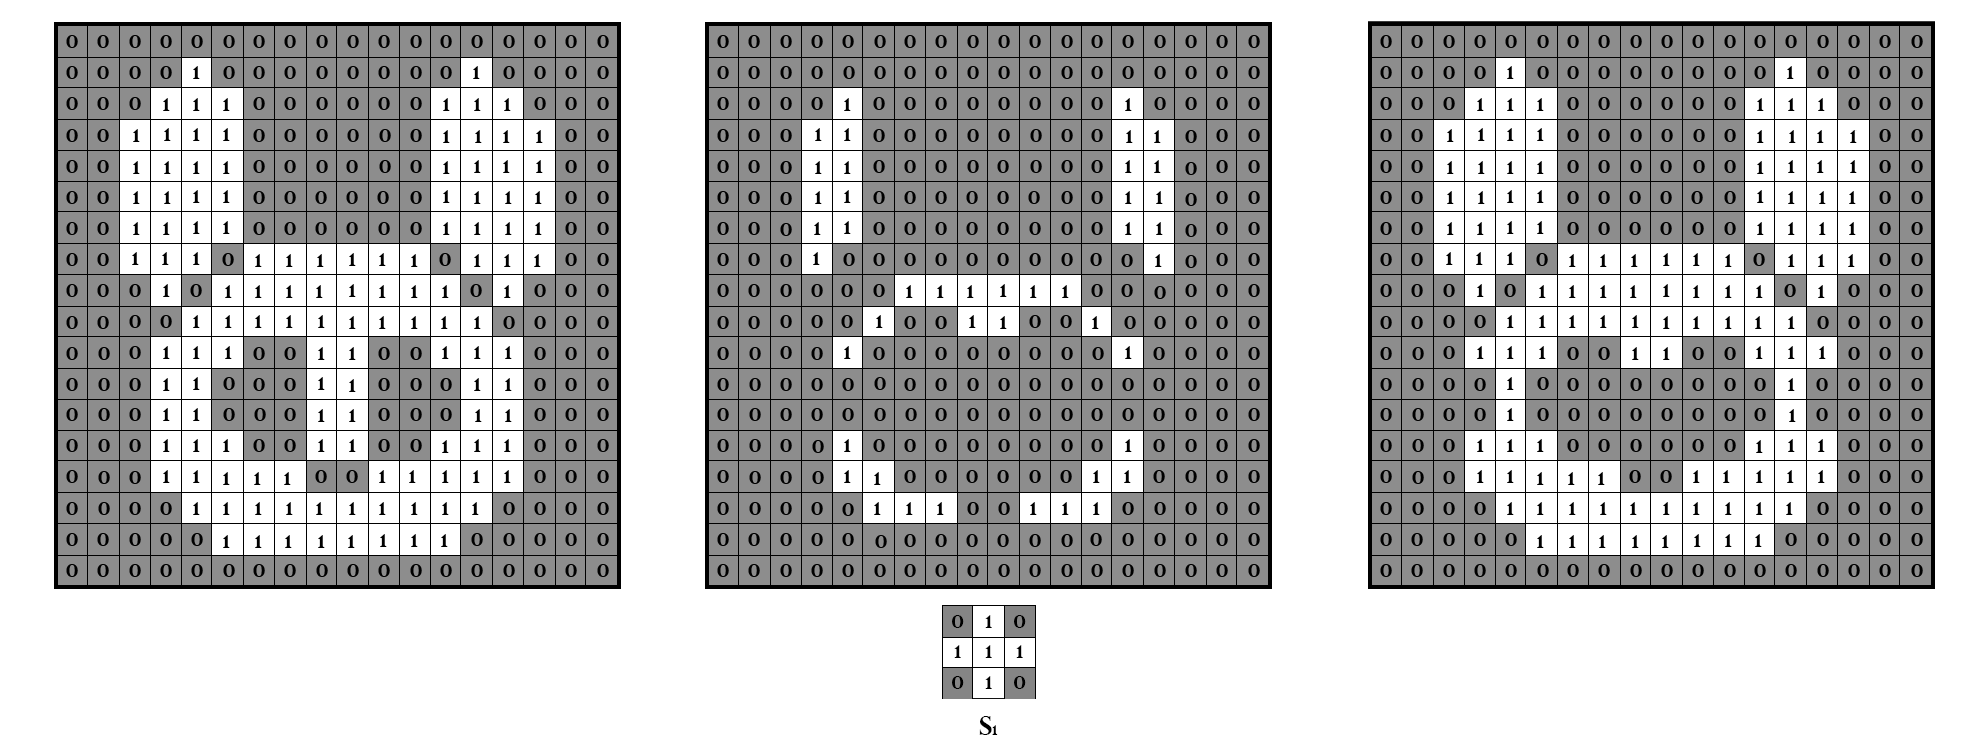
\includegraphics[width=1\textwidth]{Pictures/Theory/OpeningCirc.png}
\caption{Opening produced by a circular structured element. Inspired by \citep{ip_book}.}
\label{fig:Opening}
\end{figure}

\subsubsection{Closing}\label{closing}
When the size of the object is increased, but it is still important to constrain the measure as well as filling the holes of the objects, a good solution is to erode after the dilation. This is denoted \textit{closing} and uses eq. \ref{Closing}. As with the opening method, the size and shape of the kernel must be the same in order to obtain the desired result.

The effect of this operation can be seen in figure \ref{fig:Closing}: even though the holes are filled and the object maintains its original size, the noise of the background is still there. Therefore, it will be necessary to apply either closing or a BLOB analysis to delete those small objects.
\begin{equation}
\begin{aligned}
{g(x,y)}={f(x,y)}\bullet{SE}=({f(x,y)}\oplus{SE})\ominus{SE}
\label{Closing}
	\end{aligned}
\end{equation}

When applying closing, most of the holes of the image will be filled, but the size of the object will be the original one. 

It should be noted that using closing and/or opening combination multiple times will not achieve a better result than doing it only once on the image. However if the same operation is applied a second time, the size of the final image will be decreased and increased respectively.

%%%%%%%%%%%%%%%%%%%%%%%%%%%%%%%%%%% IMAGE CLOSING %%%%%%%%%%%%%%%%%%%%%%%%%%%%%%%%%%%%
\begin{figure}[htbp]
\centering
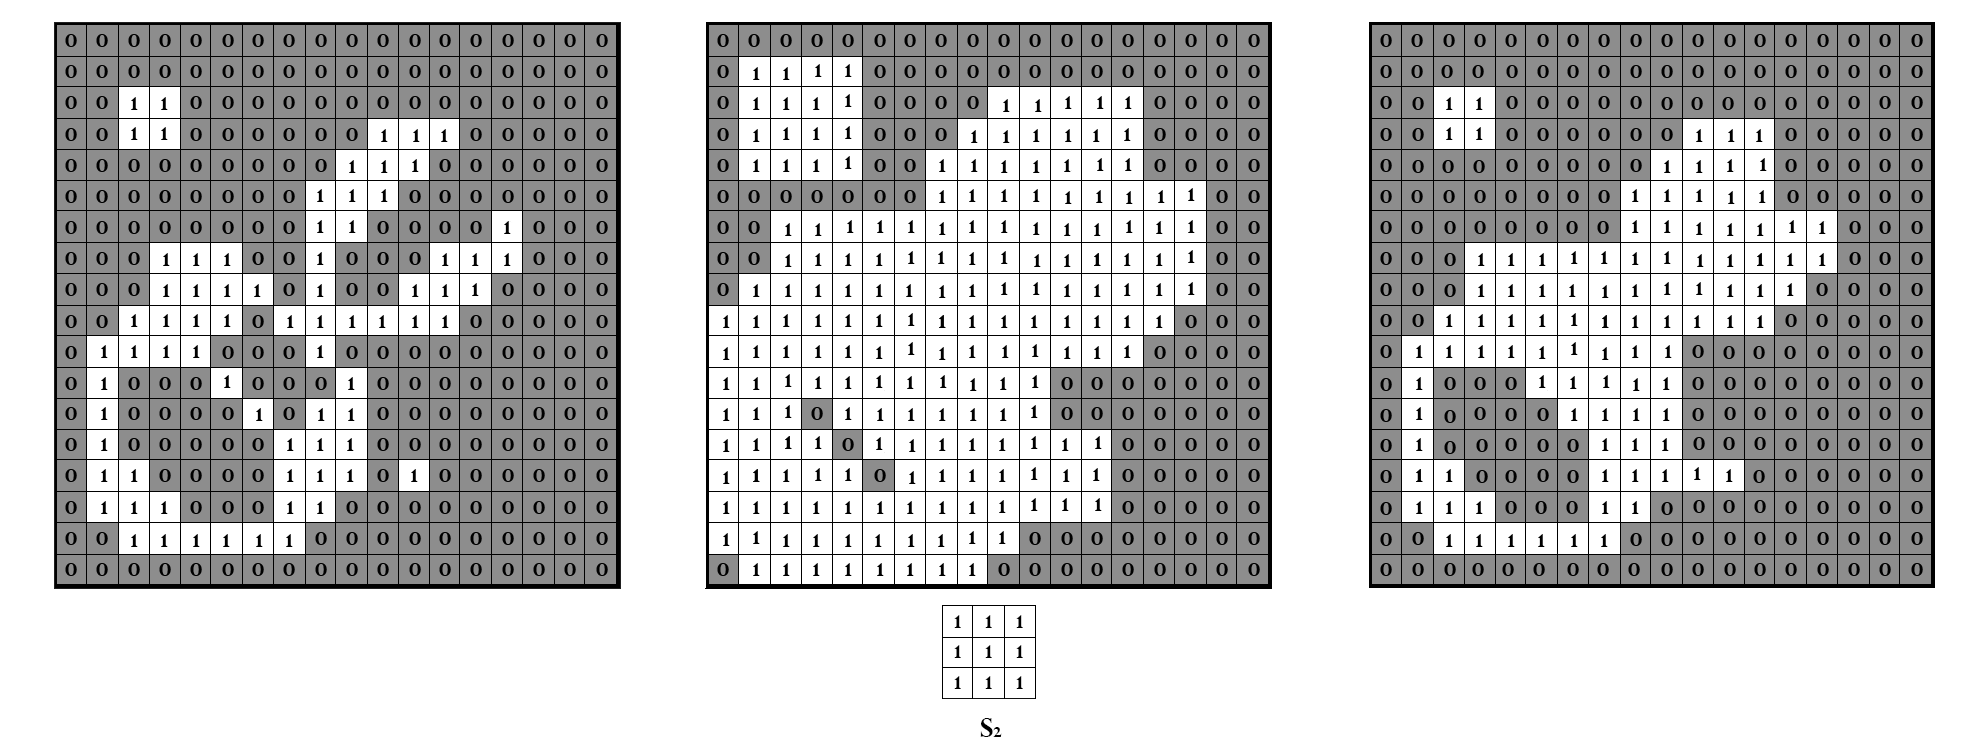
\includegraphics[width=1\textwidth]{Pictures/Theory/ClosingSq.png}
\caption{Closing produced by a squared structured element. Inspired by \citep{ip_book}.}
\label{fig:Closing}
\end{figure}

\section{Region of interest (ROI)}\label{roi}
When dealing with images some might think that more pixels are always better. However this is not always true. Since there are more pixels to loop through, it takes longer time for the computer to analyze and process the image data. The more pixels to process, the more time is required for the program to do the necessary calculations.

When working with video, it is important to maintain a stable frame rate. The more information needed to be processed, the slower the program will be. One way to ease the computational requirements is to use what is called a \textit{region of interest} (ROI). As the name suggests, the point is to choose a specific region of the image that is of interest. This could for instance be the upper part of an image where heads are expected to be. This region is usually enclosed in a rectangle and only the pixels inside this rectangle are being processed, ignoring all the pixels outside of the ROI. This prevents unnecessary processing and optimizes the speed of the program by decreasing the amount of data processed.

An example of how this could be used is taking a photo where only the head is of interest (see picture \ref{fig:Region of Interest}).

\begin{figure}[htbp] 
\centering 
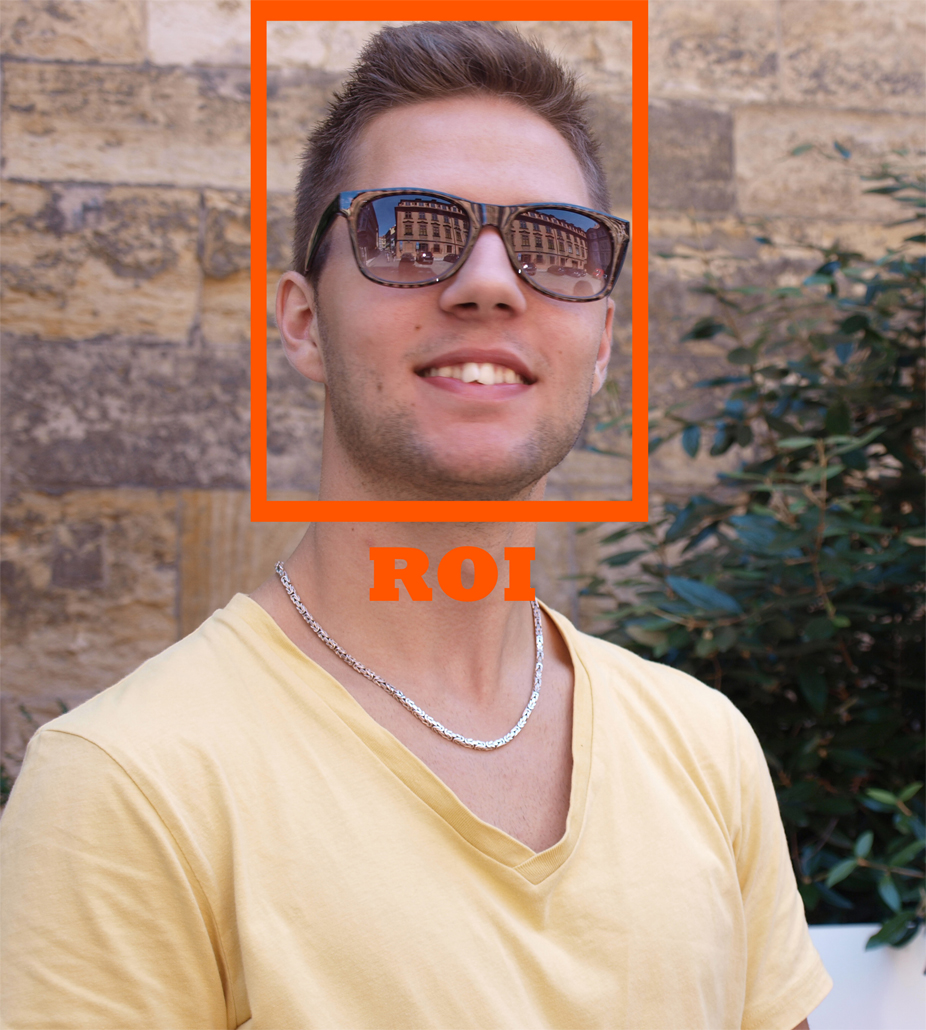
\includegraphics[width=0.5\textwidth]{Pictures/Theory/RegionOfInterest.jpg} 
\caption{Illustrating the principle of region of interest.} 
\label{fig:Region of Interest} 
\end{figure} 

\section{Filters}
A filter can be applied to an image to either remove unwanted noise or to blur the image. In most of the cases, when thresholding an image, noise appears. Noise can be in form of small dots in the background or small holes in the object of interest. By using filters on the image it is possible to remove noise. Two techniques will be described in this section: the mean and median filters.

\subsubsection{Mean filter}
One method of image filtering is the \textit{mean filter}. As the name implies, a mean filter takes an input image and calculates the mean value of a given pixel and outputs this value. This type of neighborhood processing takes the average of the input pixel and its surrounding pixels and thereby decides the value of the output pixel (see figure \ref{fig:neigh_pros}).

\begin{figure}[htbp] 
\centering 
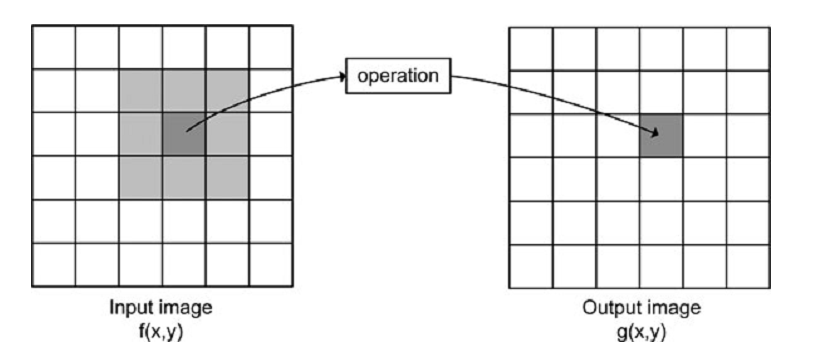
\includegraphics[width=0.5\textwidth]{Pictures/Theory/neighborhood_processing.png} 
\caption{Practical neighborhood processing. All the surrounding pixels contribute to the value of the output. From \citep{ip_book}.} 
\label{fig:neigh_pros} 
\end{figure}

The calculations behind the average is shown in equation \ref{Mean filter}.
\begin{equation}
	\begin{aligned}
	\text{Mean} = \frac{\text{Sum of input and neighboring pixels}}{\text{Number of pixels}}
	\label{Mean filter}
	\end{aligned}
\end{equation}

Mean filters are often used to blur an image, e.g. when a person's face should stay anonymous. The amount of blur depends on the kernel's size \citep{ip_book}.

\subsubsection{Median filter}
The second method is the \textit{median filter}. This works by taking the value from a pixel, as well as its surrounding neighbors and ordering them so that the lowest value appears to the most-left and the highest value to the far-right. The method outputs the value in the very middle of the list. (see \ref{Order list of pixels.}).

\begin{equation}
\begin{aligned}{
\text{Ordered list:}[1,4,17,24,\boldsymbol{42},43,52,108,235]
	\label{Order list of pixels.}}	
	\end{aligned}
\end{equation}

Median filters are good for removing noise, especially the so-called "salt and pepper noise", as shown on figure \ref{fig:salt} \citep{ip_book}.
\begin{figure}[htbp]
\centering
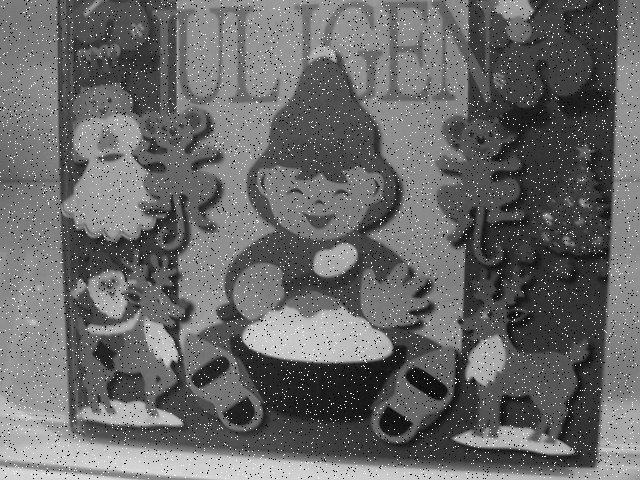
\includegraphics[width=0.5\textwidth]{Pictures/Theory/saltNoise}
\caption{A median filter can be used to remove salt and pepper noise similar to this.}
\label{fig:salt}
\end{figure}

\section{Border problem}
In neighborhood processing a kernel is applied to an image. The problem is that the kernel will always, when placed at the edge of the image, try to access pixels outside of it. Three different solutions exist to this problem, increasing the size of the output image after the neighborhood processing, increasing the size of the input image before neighborhood processing or by using special kernels for the edge-pixels.


\section{Background subtraction}
A way to detect changes in a scene and extract an object is using \textit{background subtraction}. As the name implies, it is done by subtracting the background from the scenery, so that only changes are shown.

In order to be able to use background subtraction efficiently, a controlled setup is required. The optimal setup is an indoor environment with controllable lights. This is important as the background should be static. Imagine that sunshine is let inside a room. The light will change together with the sun's position. The difference in illumination would mean that changes will be seen everywhere, which gives an inaccurate result. When doing background subtraction, it is important that the background stays the same.

%It is not realistic that each pixel in the background keeps the exact same pixel-value at all times. Therefore a threshold value is required for two main reasons. First of all to make the changes in the scene more distinct from the background, but also to have a threshold value in which the background may vary.

\section{BLOB analysis}\label{blob}
A common task when dealing with images is determining if the image contains a particular object or shape. The term \textit{BLOB} is an acronym for Binary Large Object and refers to a region of connected pixels in a binary image \citep{ip_book}. This technique can be used to extract meaningful information from images. It can be achieved by separating the pixels in points or regions that differ in properties, like brightness, color or differences compared to the background.

The process of BLOB analysis will be split in three main steps: \textit{extraction} of the BLOBs, \textit{representation} of the BLOBs and lastly, \textit{classification} of the BLOBs \citep{ip_book}.

\subsection{BLOB extraction}
To isolate BLOBs in a binary image, we need to know if two pixels are connected or not. This is done by applying algorithms that will help to determine the connectivity of the pixels, but also the number of BLOBs contained in an image. The most commonly-used kernels in BLOB extraction are the 8-connectivity and the 4-connectivity kernels \citep{ip_book}. As the 8-connectivity kernel checks for more connectivity, it requires more computations.

\subsubsection{Grass-fire algorithm}
One of these connected component labelling algorithms is the \textit{recursive grass-fire algorithm}, used to label the regions of foreground pixels to separate the BLOBs from the background.
To explain this algorithm, we will use both 8-connectivity and 4-connectivity kernels to illustrate how these choices can affect to the final result. The algorithm is denoted as recursive because it is contained within a function that calls itself \cite{ip_book}.


\begin{figure}[htbp]
\centering
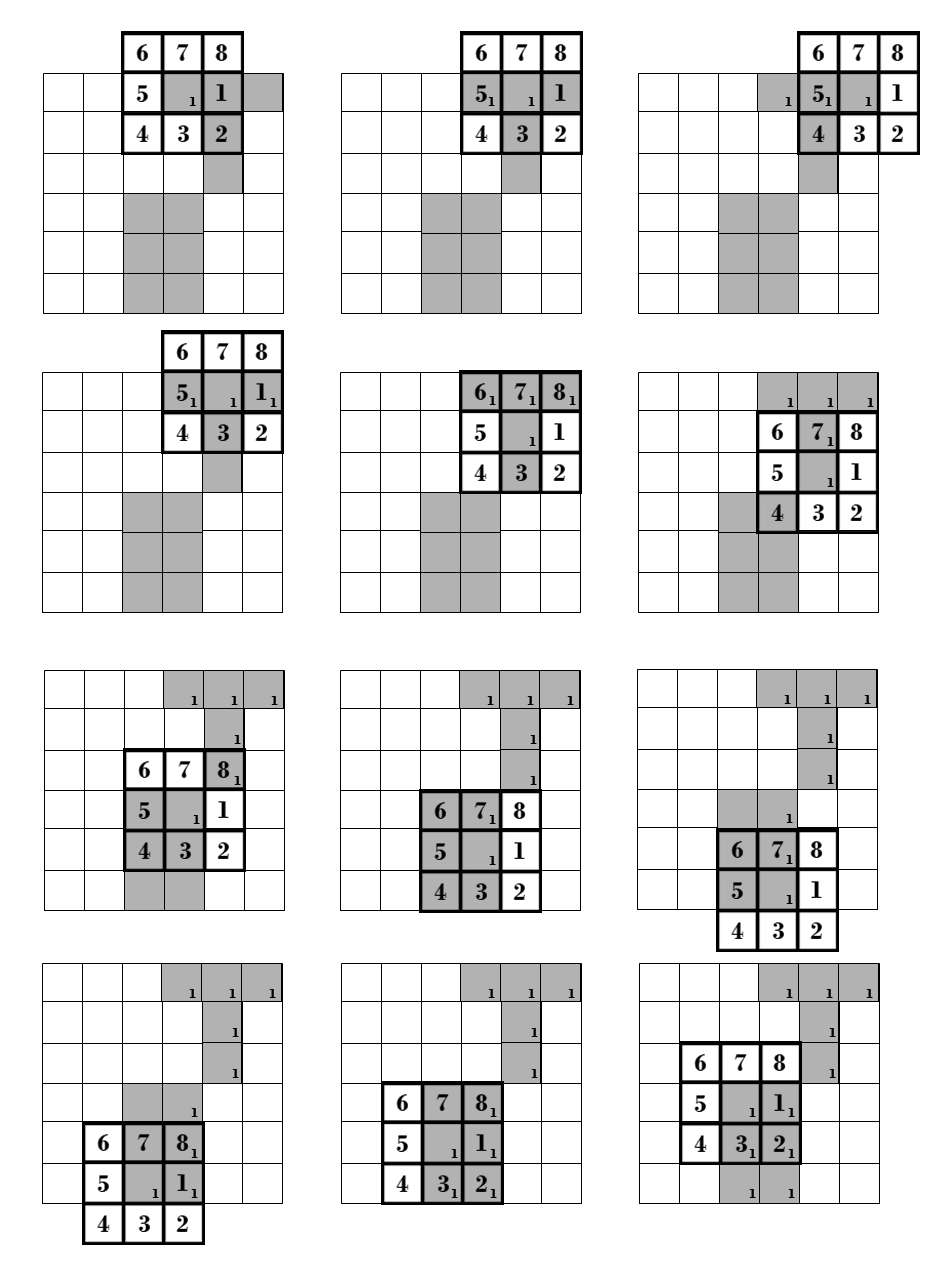
\includegraphics[width=0.8\textwidth]{Pictures/Theory/8connec_kernel.png}
\caption{8-connectivity labelling kernel detects a single object. Inspired by \citep{ip_book}.}
\label{fig:8connecK}
\end{figure}

As shown in figure \ref{fig:8connecK}, the grass-fire algorithm scans the entire image from the upper-left corner to the bottom right, row by row. When the kernel encounters a non-zero pixel value, it centers on it and "burns" the center pixel. Then the algorithm looks in the possible directions around that pixel to check if the surrounding pixels are connected to the burned pixel. The way the algorithm will do this will depend on the connectivity used (for a 8-connected kernel, the algorithm will look in 8 directions, but for the 4-connected kernel, the algorithm will look in 4 directions).

Whenever it finds an object, the algorithm labels the pixel in the output image and then burns that pixel on the input image, in order to turn it into a zero and ensure that the pixel will not be part of a new grassfire.

The algorithm now looks to the possible directions around the new pixel, starting with the pixel on the right. This process is represented on figure \ref{fig:8connecK}. Once it finds a non-zero pixel value, the algorithm once again centers its attention on it and repeats the process, labelling the pixel with the number of the previous one. At the end of that row the algorithm will check the surrounding pixels on the row below. If a non-zero pixel value is found, the algorithm will continue the process of burning and labelling pixels, otherwise the algorithm will start its way back to the beginning checking the surrounding pixels one by one to verify that it has checked all the possible directions and non-zero pixels values.

Comparing figures \ref{fig:8connecK} and \ref{fig:4connecK}, we can realize how the choice of a certain kernel will affect the final result of the algorithm using the same picture. The 8-connectivity kernel is unable to separate the different objects as intended in this particular case, whereas the 4-connectivity kernel finds the different objects performing less operations.

\begin{figure}[htbp]
\centering
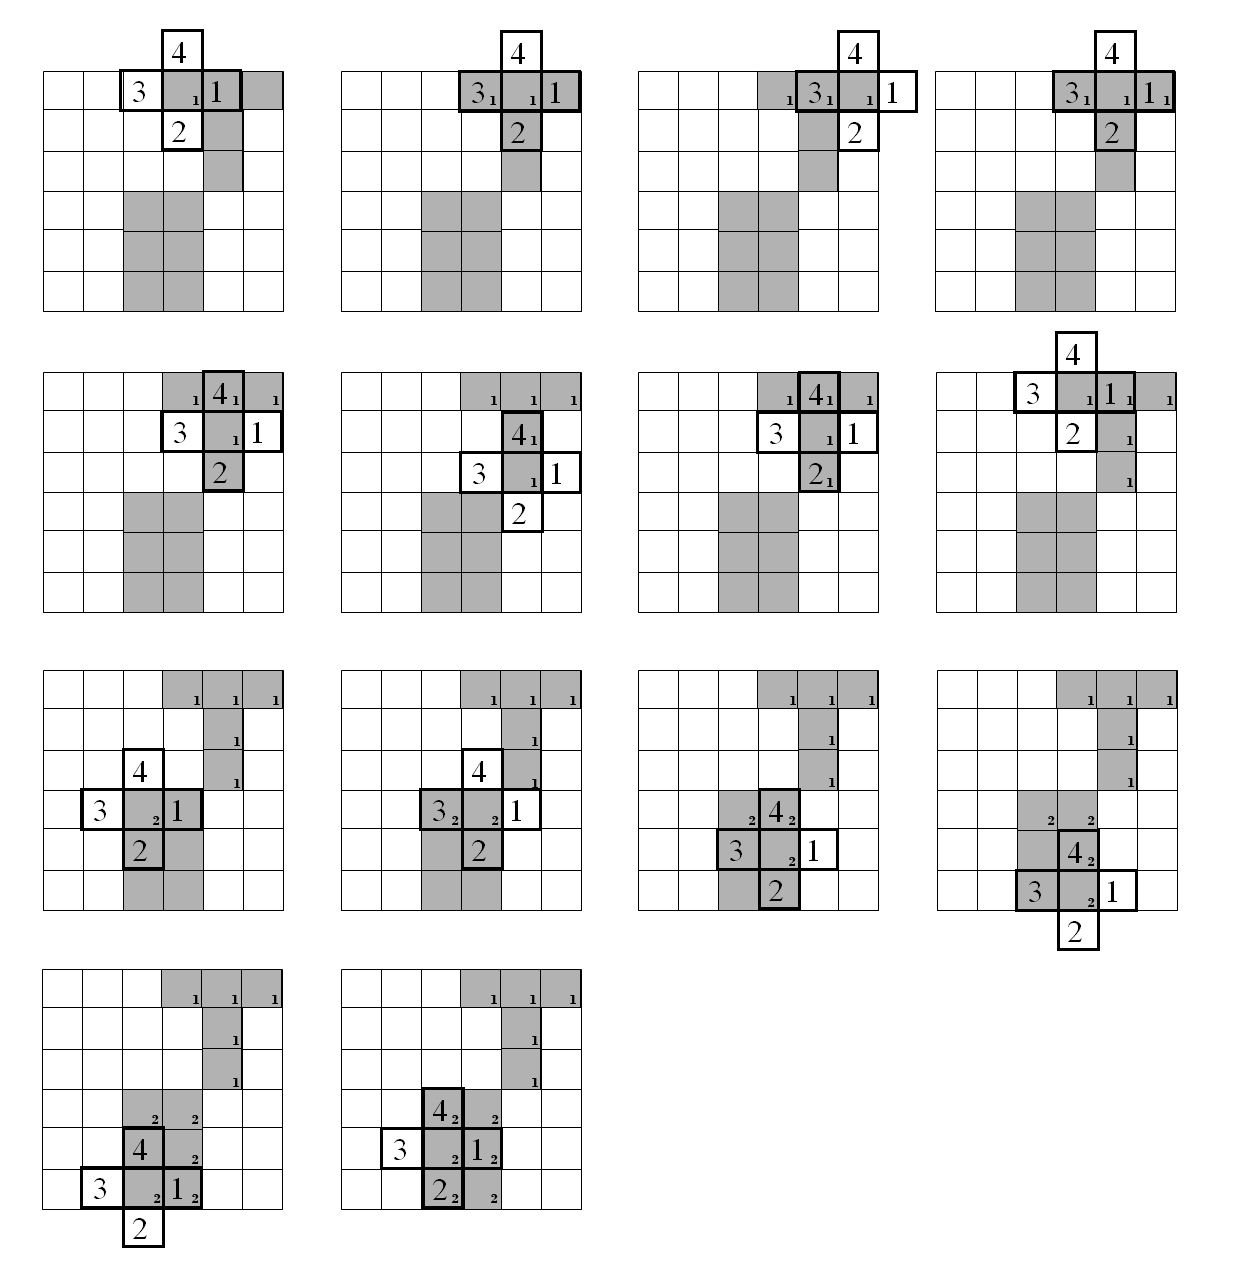
\includegraphics[width=0.75\textwidth]{Pictures/Theory/4connec_kernel.png}
\caption{4-connectivity labelling kernel detects two objects. Inspired by \citep{ip_book}.}
\label{fig:4connecK}
\end{figure}

\subsection{BLOB representation}
When looking for several different features, the classification of the BLOBs can be made by creating a prototype model of the object that we are looking for. This will allow to state the features that the BLOBs should contain, and the deviations that would be acceptable. This process consists of two steps: determining the features of the BLOBs; and matching the features with the prototype to determine if they belong to the expect ones. Still, a few features like the area, the perimeter and the circularity can already help classifying the BLOBs \citep{ip_book}.

\subsubsection{The features}

\begin{itemize}
\item \textbf{Area}
The importance of calculating features like the area of a BLOB is well understood since one of the first steps while classifying the detected objects is to delete those that are bigger or smaller than the prototype. One way of doing this is by calculating the area of the BLOB.
\item \textbf{Perimeter}
Scanning along the border of the BLOB and summing the pixels, we obtain the length of the contour of the BLOB. In image processing, this could be done by using morphology techniques like erosion to get a smaller version of the object and then subtracting this to the input image in order to get the edges.
\item \textbf{Circularity}
Circularity is a common shape-factor that depends on the perimeter and the area. There are several ways to define how circular an object can be, but usually applying the ratio to get a value lower or equal to 1 will indicate how circular the BLOB is, where 1 is a complete circle.
\end{itemize}

After all the features are extracted, a binary object can be defined by its features' values that would be stored into a feature vector in order to have a list where to start the BLOB classification.

% IMAGE WITH OBJECTS AND TABLE WITH DATA

\begin{figure}[ht]
\begin{minipage}[b]{0.45\linewidth}
\centering
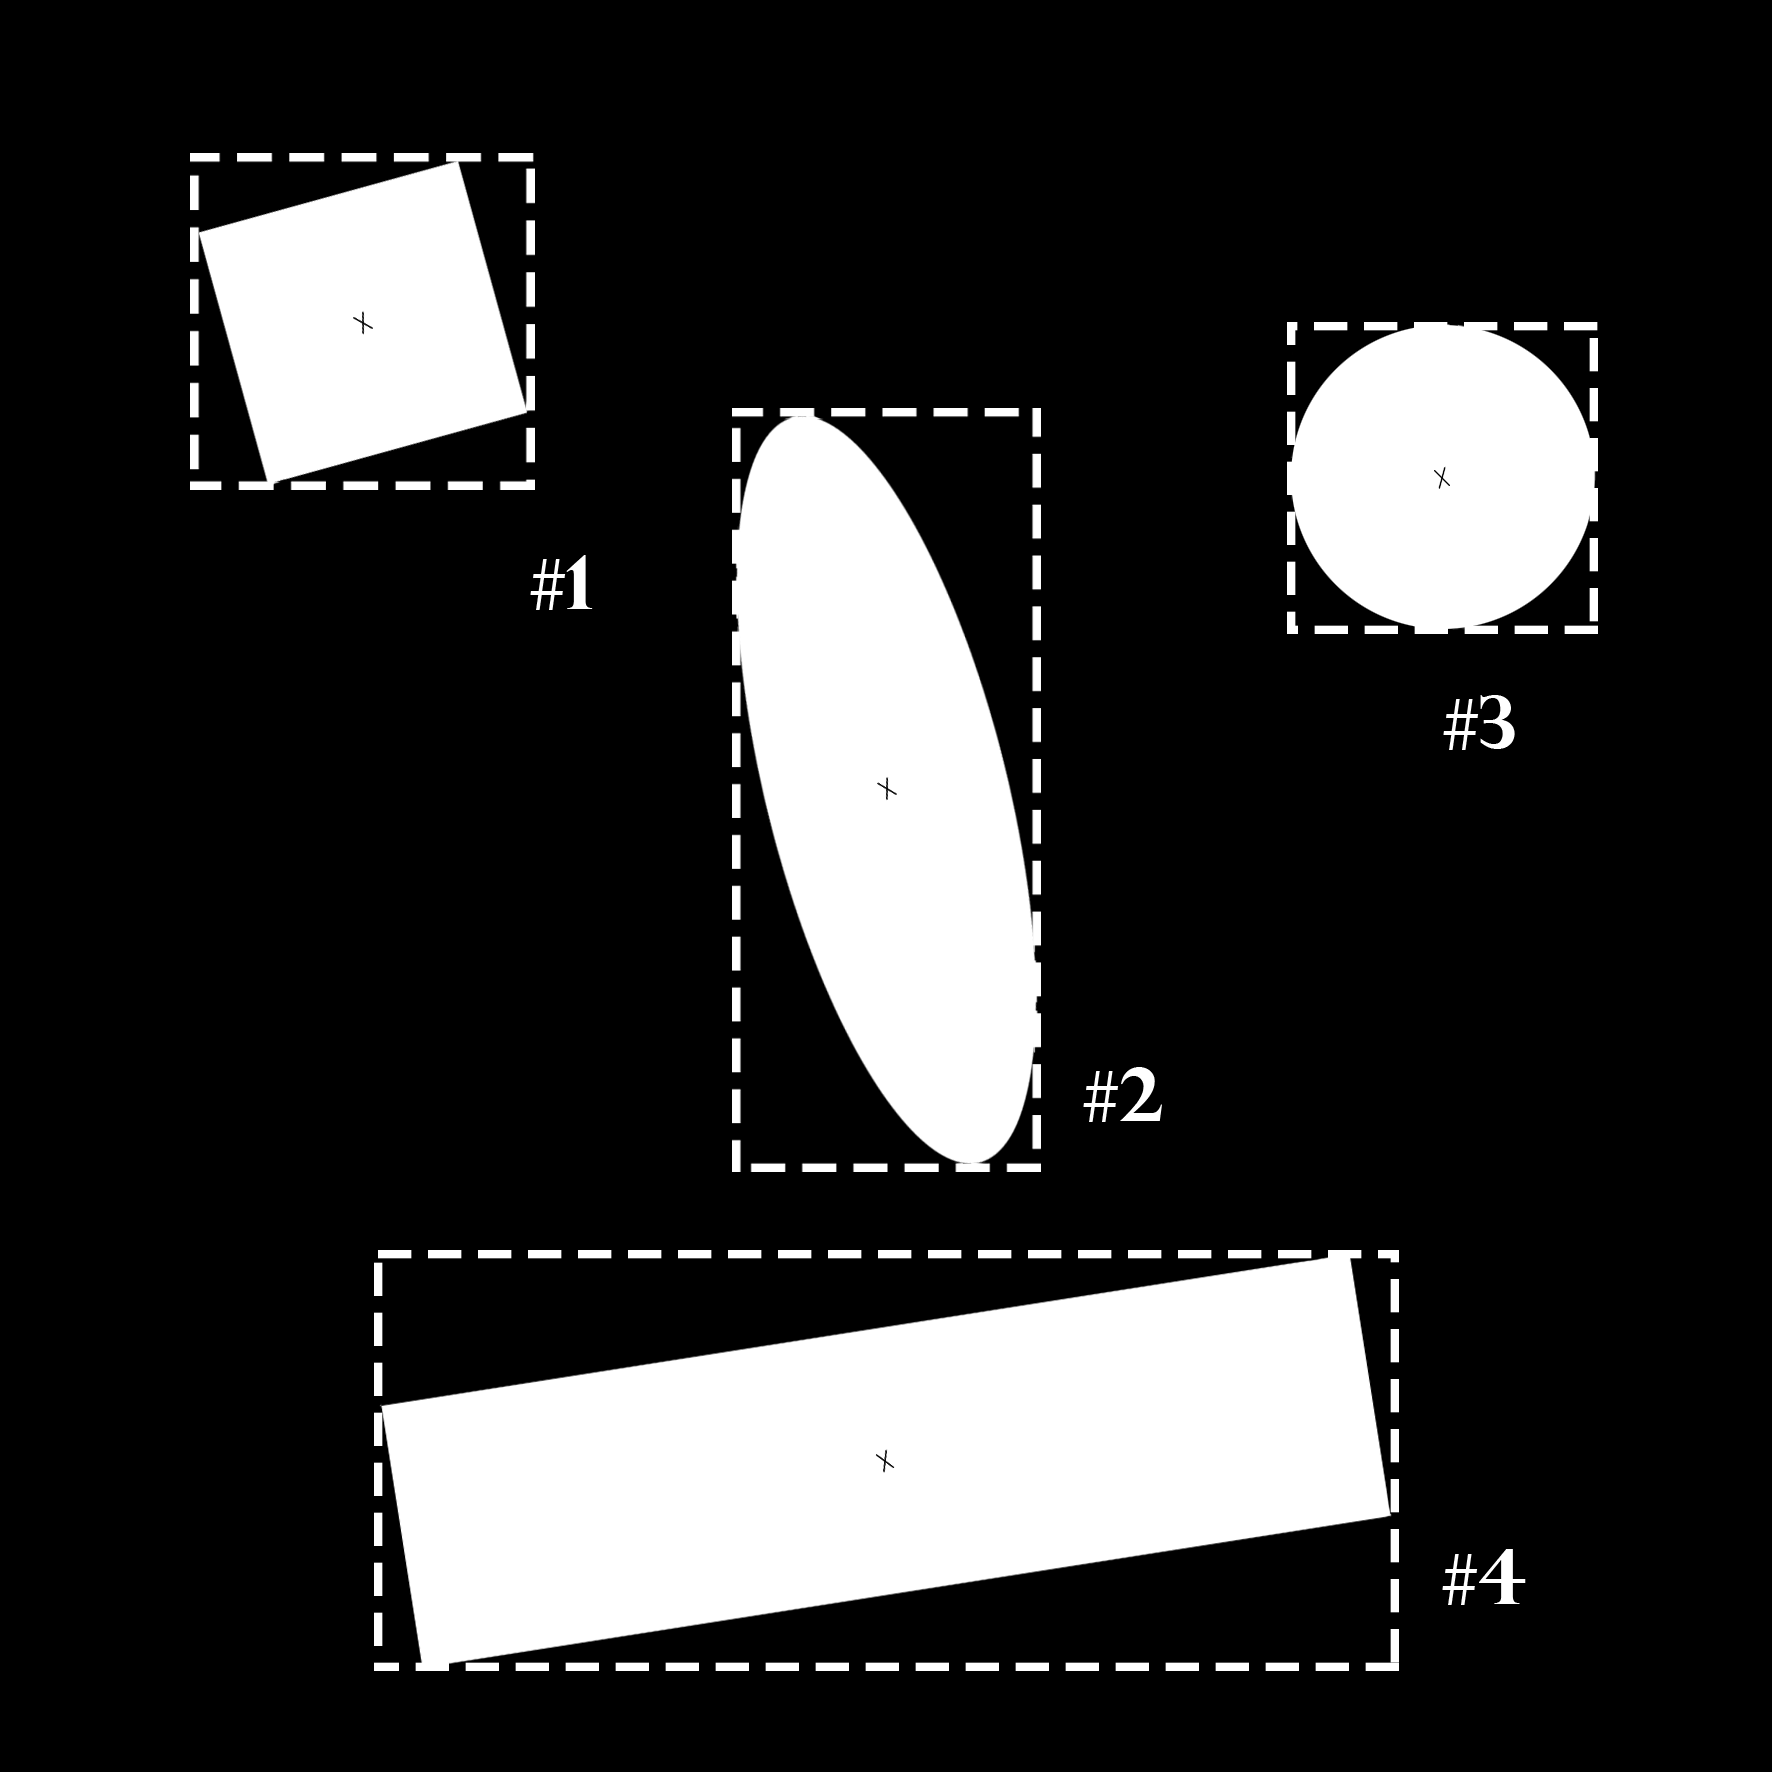
\includegraphics[width=1\textwidth]{Pictures/Theory/binary_image.png}
\end{minipage}
\hspace{0.5cm}	
\begin{minipage}[b]{0.45\linewidth}
\centering
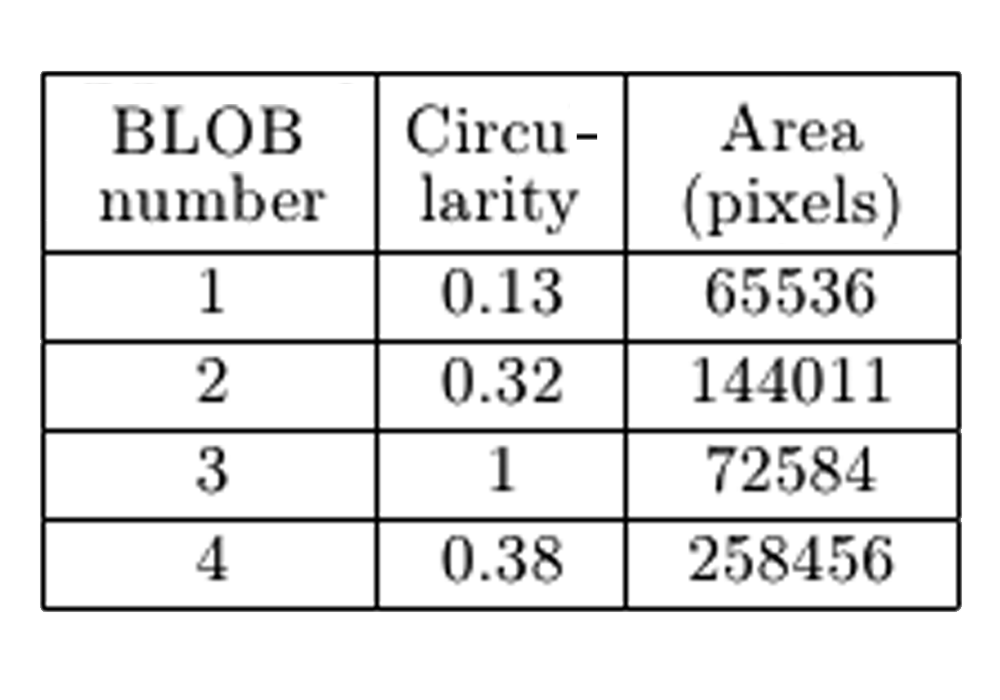
\includegraphics[width=1\textwidth]{Pictures/Theory/binary_image_table.png}
\end{minipage}
\label{fig:BinaryIm}
\caption{Binary image with a bounding box and the center-of-mass. The table shows two other features that can be calculated: the perimeter and the area. Inspired by \citep{ip_book}.}
\end{figure}

%%%%%%%%%%%%%%%%%%%%%%%%%%%%%%%%%%%%%%%%%%%%%%%%%%%%%%%%%%%%%%%%%%%%%%%%%%%%%%%%

\subsection{BLOB classification}
Once the BLOBs are extracted, their features will be used to determine if they are the BLOBs looked for. Further more, one can use the found features to build a \textit{prototype model}. This prototype model is used to keep track of more complex features like circularity or combined features. As some extracted features will not fit perfectly the prototype model features, a deviation will still be acceptable.